%% Creator: Inkscape 0.48.5, www.inkscape.org
%% PDF/EPS/PS + LaTeX output extension by Johan Engelen, 2010
%% Accompanies image file 'whittledhist.pdf' (pdf, eps, ps)
%%
%% To include the image in your LaTeX document, write
%%   \input{<filename>.pdf_tex}
%%  instead of
%%   \includegraphics{<filename>.pdf}
%% To scale the image, write
%%   \def\svgwidth{<desired width>}
%%   \input{<filename>.pdf_tex}
%%  instead of
%%   \includegraphics[width=<desired width>]{<filename>.pdf}
%%
%% Images with a different path to the parent latex file can
%% be accessed with the `import' package (which may need to be
%% installed) using
%%   \usepackage{import}
%% in the preamble, and then including the image with
%%   \import{<path to file>}{<filename>.pdf_tex}
%% Alternatively, one can specify
%%   \graphicspath{{<path to file>/}}
%% 
%% For more information, please see info/svg-inkscape on CTAN:
%%   http://tug.ctan.org/tex-archive/info/svg-inkscape
%%
\begingroup%
  \makeatletter%
  \providecommand\color[2][]{%
    \errmessage{(Inkscape) Color is used for the text in Inkscape, but the package 'color.sty' is not loaded}%
    \renewcommand\color[2][]{}%
  }%
  \providecommand\transparent[1]{%
    \errmessage{(Inkscape) Transparency is used (non-zero) for the text in Inkscape, but the package 'transparent.sty' is not loaded}%
    \renewcommand\transparent[1]{}%
  }%
  \providecommand\rotatebox[2]{#2}%
  \ifx\svgwidth\undefined%
    \setlength{\unitlength}{800bp}%
    \ifx\svgscale\undefined%
      \relax%
    \else%
      \setlength{\unitlength}{\unitlength * \real{\svgscale}}%
    \fi%
  \else%
    \setlength{\unitlength}{\svgwidth}%
  \fi%
  \global\let\svgwidth\undefined%
  \global\let\svgscale\undefined%
  \makeatother%
  \begin{picture}(1,0.4)%
    \put(0,0){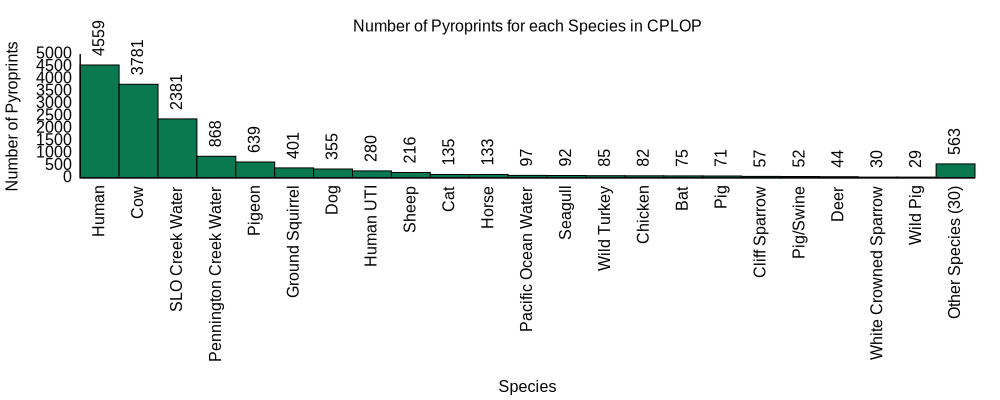
\includegraphics[width=\unitlength]{whittledhist.pdf}}%
    \put(0.0719,0.2177){\makebox(0,0)[rb]{\smash{0}}}%
    \put(0.0719,0.2301){\makebox(0,0)[rb]{\smash{500}}}%
    \put(0.0719,0.2424){\makebox(0,0)[rb]{\smash{1000}}}%
    \put(0.0719,0.2548){\makebox(0,0)[rb]{\smash{1500}}}%
    \put(0.0719,0.2672){\makebox(0,0)[rb]{\smash{2000}}}%
    \put(0.0719,0.2796){\makebox(0,0)[rb]{\smash{2500}}}%
    \put(0.0719,0.2919){\makebox(0,0)[rb]{\smash{3000}}}%
    \put(0.0719,0.3043){\makebox(0,0)[rb]{\smash{3500}}}%
    \put(0.0719,0.3167){\makebox(0,0)[rb]{\smash{4000}}}%
    \put(0.0719,0.329){\makebox(0,0)[rb]{\smash{4500}}}%
    \put(0.0719,0.3414){\makebox(0,0)[rb]{\smash{5000}}}%
    \put(0.1042,0.2139){\rotatebox{90}{\makebox(0,0)[rb]{\smash{Human}}}}%
    \put(0.1431,0.2139){\rotatebox{90}{\makebox(0,0)[rb]{\smash{Cow}}}}%
    \put(0.182,0.2139){\rotatebox{90}{\makebox(0,0)[rb]{\smash{SLO Creek Water}}}}%
    \put(0.2209,0.2139){\rotatebox{90}{\makebox(0,0)[rb]{\smash{Pennington Creek Water}}}}%
    \put(0.2598,0.2139){\rotatebox{90}{\makebox(0,0)[rb]{\smash{Pigeon}}}}%
    \put(0.2987,0.2139){\rotatebox{90}{\makebox(0,0)[rb]{\smash{Ground Squirrel}}}}%
    \put(0.3376,0.2139){\rotatebox{90}{\makebox(0,0)[rb]{\smash{Dog}}}}%
    \put(0.3765,0.2139){\rotatebox{90}{\makebox(0,0)[rb]{\smash{Human UTI}}}}%
    \put(0.4154,0.2139){\rotatebox{90}{\makebox(0,0)[rb]{\smash{Sheep}}}}%
    \put(0.4543,0.2139){\rotatebox{90}{\makebox(0,0)[rb]{\smash{Cat}}}}%
    \put(0.4932,0.2139){\rotatebox{90}{\makebox(0,0)[rb]{\smash{Horse}}}}%
    \put(0.5321,0.2139){\rotatebox{90}{\makebox(0,0)[rb]{\smash{Pacific Ocean Water}}}}%
    \put(0.571,0.2139){\rotatebox{90}{\makebox(0,0)[rb]{\smash{Seagull}}}}%
    \put(0.6099,0.2139){\rotatebox{90}{\makebox(0,0)[rb]{\smash{Wild Turkey}}}}%
    \put(0.6488,0.2139){\rotatebox{90}{\makebox(0,0)[rb]{\smash{Chicken}}}}%
    \put(0.6877,0.2139){\rotatebox{90}{\makebox(0,0)[rb]{\smash{Bat}}}}%
    \put(0.7266,0.2139){\rotatebox{90}{\makebox(0,0)[rb]{\smash{Pig}}}}%
    \put(0.7655,0.2139){\rotatebox{90}{\makebox(0,0)[rb]{\smash{Cliff Sparrow}}}}%
    \put(0.8044,0.2139){\rotatebox{90}{\makebox(0,0)[rb]{\smash{Pig/Swine}}}}%
    \put(0.8433,0.2139){\rotatebox{90}{\makebox(0,0)[rb]{\smash{Deer}}}}%
    \put(0.8822,0.2139){\rotatebox{90}{\makebox(0,0)[rb]{\smash{White Crowned Sparrow}}}}%
    \put(0.9211,0.2139){\rotatebox{90}{\makebox(0,0)[rb]{\smash{Wild Pig}}}}%
    \put(0.96,0.2139){\rotatebox{90}{\makebox(0,0)[rb]{\smash{Other Species (30)}}}}%
    \put(0.0176,0.284){\rotatebox{90}{\makebox(0,0)[b]{\smash{Number of Pyroprints}}}}%
    \put(0.5276,0.0081){\makebox(0,0)[b]{\smash{Species}}}%
    \put(0.5276,0.3684){\makebox(0,0)[b]{\smash{Number of Pyroprints for each Species in CPLOP}}}%
    \put(0.1042,0.344){\rotatebox{90}{\makebox(0,0)[lb]{\smash{4559}}}}%
    \put(0.1431,0.3247){\rotatebox{90}{\makebox(0,0)[lb]{\smash{3781}}}}%
    \put(0.182,0.2901){\rotatebox{90}{\makebox(0,0)[lb]{\smash{2381}}}}%
    \put(0.2209,0.2527){\rotatebox{90}{\makebox(0,0)[lb]{\smash{868}}}}%
    \put(0.2598,0.247){\rotatebox{90}{\makebox(0,0)[lb]{\smash{639}}}}%
    \put(0.2987,0.2411){\rotatebox{90}{\makebox(0,0)[lb]{\smash{401}}}}%
    \put(0.3376,0.24){\rotatebox{90}{\makebox(0,0)[lb]{\smash{355}}}}%
    \put(0.3765,0.2381){\rotatebox{90}{\makebox(0,0)[lb]{\smash{280}}}}%
    \put(0.4154,0.2365){\rotatebox{90}{\makebox(0,0)[lb]{\smash{216}}}}%
    \put(0.4543,0.2345){\rotatebox{90}{\makebox(0,0)[lb]{\smash{135}}}}%
    \put(0.4932,0.2345){\rotatebox{90}{\makebox(0,0)[lb]{\smash{133}}}}%
    \put(0.5321,0.2336){\rotatebox{90}{\makebox(0,0)[lb]{\smash{97}}}}%
    \put(0.571,0.2335){\rotatebox{90}{\makebox(0,0)[lb]{\smash{92}}}}%
    \put(0.6099,0.2333){\rotatebox{90}{\makebox(0,0)[lb]{\smash{85}}}}%
    \put(0.6488,0.2332){\rotatebox{90}{\makebox(0,0)[lb]{\smash{82}}}}%
    \put(0.6877,0.2331){\rotatebox{90}{\makebox(0,0)[lb]{\smash{75}}}}%
    \put(0.7266,0.233){\rotatebox{90}{\makebox(0,0)[lb]{\smash{71}}}}%
    \put(0.7655,0.2326){\rotatebox{90}{\makebox(0,0)[lb]{\smash{57}}}}%
    \put(0.8044,0.2325){\rotatebox{90}{\makebox(0,0)[lb]{\smash{52}}}}%
    \put(0.8433,0.2323){\rotatebox{90}{\makebox(0,0)[lb]{\smash{44}}}}%
    \put(0.8822,0.2319){\rotatebox{90}{\makebox(0,0)[lb]{\smash{30}}}}%
    \put(0.9211,0.2319){\rotatebox{90}{\makebox(0,0)[lb]{\smash{29}}}}%
    \put(0.96,0.2451){\rotatebox{90}{\makebox(0,0)[lb]{\smash{563}}}}%
  \end{picture}%
\endgroup%
